\chapter{Interpretazione astratta}
\section{Introduzione}
Nelle analisi precedenti l'approccio all'analisi statica è basato sull'informazione che
vogliamo osservare dell'esecuzione del programma, in particolare per proprietà relativamente semplici,
molto vicine alla sintassi che non descrivono informazioni sul contenuto delle variabili,
quindi in relazione agli elementi del programma piuttosto che al contenuto di tali elementi.

Per questo tipo di analisi, o in modo algoritmico fornendo direttamente l'equazione da risolvere, o 
in modo semantico, fornendo una semantica di elaborazione dell'informazione, costruita 
in modo induttivo sulla sintassi del linguaggio, riusciamo a fornire una soluzione sull'informazione
ricercata.

Il problema si pone quando vogliamo guardare ciò che accade al programma durante l'esecuzione, 
siamo quindi interessati a guardare all'interno delle stato della macchina, e non più alla relazione 
tra gli elementi del programma. Questo diventa relativamente un problema, poiché fornendo una 
semantica, tale semantica non risulterebbe distributiva, di conseguenza ci sarà necessariamente 
una perdita di informazione legata al fatto che risolvendo l'analisi localmente su punti di programma 
del \texttt{CFG} perdiamo informazione rispetto alla semantica desiderata, ovvero quella che considera 
tutti i cammini di esecuzione, ovvero la \textbf{MOP}. Si tratta del prezzo da pagare per rendere 
decidibile un calcolo su un informazione che si avvicina sempre di più all'informazione concreta, ovvero 
l'evoluzione dello stato della macchina.

Guardare all'interno dello stato della macchina significa avvicinarsi sempre di più 
all'informazione concreta, ma richiede un prezzo che è quello di staccarci 
dalla soluzione \textbf{MOP}, ottenendo attraverso la soluzione del calcolo 
di un sistema di disequazioni, una soluzione approssimata.

Nel momento in cui siamo interessati a guardare all'interno dello stato della macchina,
allora abbiamo bisogno, per mantenere delle garanzie sul calcolo della semantica astratta, 
di un'infrastruttura chiamata \textbf{interpretazione astratta}.

\begin{tcolorbox}[title=Interpretazione astratta]
    L'interpretazione astratta è un framework formale che permette di descrivere 
    dettagliatamente la relazione tra il momento concreto, di cui vogliamo dire 
    qualcosa, e il momento astratto, su cui possiamo dire qualcosa, garantendo informazioni 
    certe, anche se approssimate, su alcuni aspetti di interesse
    del mondo concreto.
\end{tcolorbox}
L'obiettivo è di verificare in modo automatico proprietà di interesse dei programmi e 
l'astrazione è il procedimento utilizzato per arginare il problema della non decidibilità
della semantica concreta.

\section{L'idea di base dell'interpretazione astratta}
L'idea di base è che un qualunque oggetto concreto sia formato da due elementi, un origine e 
un insieme finito di punti.

Supponiamo di definire nel nostro dominio concreto un oggetto fiore e vediamo come è possibile 
ottenerlo attraverso l'applicazione di operazioni concrete e partendo da operazioni concrete.
\begin{figure}[H]
    \centering 
    \includegraphics[scale=0.5]{img/flower.png}
\end{figure}
Tali oggetti non sono altro che dei numeri interni, quindi immaginiamo il fiore come una sequenza 
di operazioni che applichiamo ad elementi più piccoli, ovvero elementi del dominio stesso.
\subsection{Operazioni concrete}
Le operazioni che possiamo applicare sono le seguenti:
\begin{itemize}
    \item Costante: operazione che fornisce un petalo.
    \item Rotazione: $r[a](o)$ è un'operazione che ruota di $a$ gradi l'oggetto $o$.
    \begin{figure}[H]
        \centering 
        \includegraphics[scale=0.5]{img/rotation.png}
    \end{figure}
    \item Unione: $o_1 \cup o_2$ è un'operazione che unisce due oggetti $o_1$ e $o_2$, sovrapponendo 
    le origini.
    \begin{figure}[H]
        \centering 
        \includegraphics[scale=0.5]{img/corolla.png}
        \caption{$\texttt{corolla} = \texttt{petal} \cup r[45]\texttt{petal} 
        \cup r[90]\texttt{petal} \cup r[135]\texttt{petal}
        \cup r[180]\texttt{petal} \cup r[225]\texttt{petal} 
        \cup r[270]\texttt{petal} \cup r[315]\texttt{petal}$}
    \end{figure}
    \item \textit{stem}(o): è un'operazione che aggiunge un gambo all'oggetto $o$, il gambo viene sovrapposto 
    all'origine e la nuova origine è quella del gambo.
    \begin{figure}[H]
        \centering 
        \includegraphics[scale=0.5]{img/stem.png}
    \end{figure}
\end{itemize}
Per la costruzione della corolla possiamo trovare un operatore monotono che applicato iterativamente 
fino al raggiungimento di un punto fisso, ci permette di ottenere la corolla. Possiamo costruire oggetti 
concreti per punto fisso a partire da oggetti più semplici, che è ciò che avviene con la semantica.
\[
  \texttt{corolla} = lfp^{\subseteq} F  
\]
\[
    F(X) = \texttt{petal} \cup r[45](X)
\]
\begin{figure}[H]
    \centering
    \includegraphics[scale=0.5]{img/fixpointcorolla.png}
\end{figure}
Abbiamo quindi introdotto un dominio concreto di oggetti su cui abbiamo definito delle operazioni.
\subsection{Approssimazione verso l'alto}
Operare su tali oggetti può comportare situazioni di non decidibilità, l'idea è quindi di approssimare 
tali oggetti concreti.
Definiamo la relazione di approssimazione, ovvero cosa vuol dire essere meno precisi. Nel caso degli 
oggetti, quello che è essere meno precisi è avere la stessa origine, ma che contengono più pixel, ovvero 
aggiungere rumore rispetto all'informazione originale.
\begin{figure}[H]
    \centering
    \includegraphics[scale=0.5]{img/upperapprox.png}
\end{figure}
In questo particolare caso abbiamo perso parte del dettaglio della figura, in particolare la corolla.
Aver più pixel aggiunge quindi rumore.

\subsection{Oggetti astratti}
L'oggetto astratto è una rappresentazione di un oggetto concreto che vogliamo fornire in 
forma approssimata. Decidiamo di rappresentare l'insieme di pixel dal suo contorno.
Questo è l'ordine che inseriamo nel dominio di computazione, propagando l'ordinamento,
che nel dominio concreto è dato dal contenimento, sul dominio astratto.
Un oggetto è quindi più astratto se è la rappresentazione di un oggetto concreto più grande.
\begin{figure}[H]
    \centering
    \includegraphics[scale=0.6]{img/abstractobj.png}
\end{figure}
L'idea è che il contorno di un certo oggetto venga disegnato con una pennarello 
di spessore variabile, la variabilità di tale spessore è data dal livello di astrazione.
Disegnando un un pennarello più spesso, si perde dettaglio, mentre disegnando
con un pennarello più sottile, si guadagna dettaglio.

\begin{tcolorbox}[title = Dominio astratto]
    Il dominio astratto è l'insieme di tutti gli oggetti astratti, più 
    le operazioni astratte che permettono di costruire oggetti astratti
    (\textit{che approssimano le operazioni concrete}).
\end{tcolorbox}
\begin{tcolorbox}[title =  Astrazione]
    L'astrazione è una funzione $\alpha$ che mappa ogni oggetto concreto
    in una approssimazione rappresentata da un oggetto astratto $\alpha(o)$
    in modo univoco.
\end{tcolorbox}
Il tutto è costruito in modo tale da poter confrontare oggetti astratti 
tra di loro, scegliendo di guardare l'informazione approssimata allargando 
il diametro del pennarello.
\subsection{Concretizzazione}
Nel mondo dell'interpretazione astratta corrisponde ad assegnare il significato 
concreto dell'oggetto astratto che stiamo osservando.

Nel caso degli oggetti rappresentati precedentemente, la concretizzazione
è possibile vederla come l'idea di riempire il contorno dell'oggetto astratto.
\begin{figure}[H]
    \centering
    \includegraphics[scale=0.6]{img/concretizzazione.png}
\end{figure}
Si tratta di una funzione $\gamma$ che mappa ogni oggetto
astratto $\bar{o}$ in un oggetto concreto, in modo univoco
$\gamma(\bar{o})$.

Prendendo in considerazione l'insieme $\{2,6\}$ l'astrazione
di tale insieme, ovvero l'applicazione $\alpha$, può essere visto come la 
funzione che mappa l'insieme $\{2,6\}$ (\textit{fiore concreto}) in un oggetto astratto
che rappresenta l'insieme $2\mathbb{Z}$ (\textit{fiore astratto}). L'applicazione 
della funzione $\gamma$ su tale oggetto astratto, fa si che 
si ottenga $\{0,2,4,6,\dots\}$ (\textit{fiore riempito}).
\subsection{Connessione di Galois}
Queste due funzioni di concretizzazione e astrazione nell'interpretazione
astratta sono modellate dal concetto di \textbf{connessione di Galois}.

Dice infatti che è una coppia di funzioni, tali che:
\begin{itemize}
    \item $\alpha$ è monotona
    \begin{figure}[H]
        \centering
        \includegraphics[scale=0.6]{img/galoisconn1.png}
    \end{figure}
    \item $\gamma$ è monotona
    \begin{figure}[H]
        \centering
        \includegraphics[scale=0.6]{img/galoisconn2.png}
    \end{figure}
\end{itemize}
La monotonia fa si che preservino l'ordine tra i due domini.

In più le connessioni di Galois devono estendere quando si esegue 
il processo di astrazione, quindi il processo di astrazione può aggiungere 
rumore:
\[
    \textit{per ogni oggetto concreto } x, \gamma \circ \alpha(x) \subseteq x
\]
\begin{figure}[H]
    \centering
    \includegraphics[scale=0.6]{img/galoisconn3.png}
\end{figure}
Inoltre se prima concretizziamo e poi astraiamo, otteniamo
un oggetto astratto più piccolo di quello di partenza, questo perché 
nel mondo concreto potrebbero esserci oggetti inutili che non hanno significato.
\[
    \textit{per ogni oggetto astratto } y, \alpha \circ \gamma(y) \sqsubseteq  y
\]
Tipicamente si ha che $\alpha \circ \gamma(y) = y$.
\begin{figure}[H]
    \centering
    \includegraphics[scale=0.6]{img/galoisconn4.png}
\end{figure}
\subsection{Ordinamento astratto}
L'ordinamento astratto è il trasferimento dell'ordinamento concreto
sul dominio astratto. Quindi un oggetto astratto è più piccolo di un altro
oggetto astratto se la corrisponde concretizzazione è più piccola.
\begin{figure}[H]
    \centering
    \includegraphics[scale=0.6]{img/abstractordering.png}
\end{figure}
In origine ciò che volevamo fare era calcolare delle operazioni sul dominio concreto 
con l'assunzione che tali operazioni non fossero sempre decidibili. L'obiettivo 
è trasferire tali operazioni dal mondo concreto al mondo astratto, in modo tale
da poterle calcolare in modo sempre decidibile.
Il modo più immediato per farlo è quello di passare attraverso le operazioni concrete.
Nell'esempio del gambo abbiamo in fatti che:
\[
    \overline{\texttt{stem}} = \alpha (\texttt{stem} (\gamma(y)))
\]
\begin{figure}[H]
    \centering
    \includegraphics[scale=0.6]{img/abstractstem.png}
\end{figure}
Non potevamo aggiungere direttamente il gambo alla corolla astratta 
poiché avremmo avuto un livello di dettaglio diverso dal risultato finale 
che non avrebbe coinciso con lo spessore del pennarello scelto per 
osservare l'oggetto concreto.
È necessario definire un'operazione ad hoc per
poter lavorare su oggetti astratti, preservando quindi l'informazione che 
abbiamo sull'oggetto astratto, ovvero che il suo contorno è stato delimitato 
con un certo spessore e su tutte le operazioni è possibile eseguire 
tale passaggio.
\subsection{Punto fisso astratto}
Esattamente come le operazioni precedenti, anche il calcolo di punto fisso 
può essere trasferito dal mondo concreto a quello astratto.

Possiamo eseguire direttamente un'astrazione del punto fisso:
\[
  \texttt{abstract corolla} = \alpha(\texttt{concrete corolla}) =
    \alpha(lfp^{\subseteq} F)  
\]
Dove $F(X)= \texttt{petal} \cup r[45](X)$.
Sappiamo però che possa ereditare problemi di decidibilità 
e di convergenza, poiché il punto fisso se esiste in presenza di 
funzioni monotone, può divergere. È chiaro che poiché ci spostiamo 
nel mondo astratto per controllare questo tipo di divergenza, non avrebbe 
senso calcolare il punto fisso concreto e poi astrarlo. L'obiettivo 
è quello di costruire un operatore astratto il cui punto fisso nel mondo 
ideale che sia esattamente l'astrazione del punto fisso concreto, 
però con il fatto il punto fisso astratto è calcolato su un mondo 
approssimato e quindi potenzialmente convergente.
\[
    \alpha(lfp^{\subseteq} F) = lfp^{\sqsubseteq} \overline{F}
\]
In generale si tratta della situazione ideale, in cui abbiamo costruito 
esattamente l'operatore di punto fisso che sul nostro dominio riesce 
a raggiungere precisamente la proprietà del punto fisso concreto.
In generale quello che succede è che il punto fisso astratto sarà 
un'approssimazione ulteriore della proprietà del punto fisso concreto.

\begin{figure}[H]
    \centering
    \includegraphics[scale=0.6]{img/abstractfixpoint.png}
\end{figure}

\section{Costruzione formale dell'interpretazione astratta}
Vediamo ora gli strumenti formali che utilizziamo per modellare e 
descrivere quelle che sono le basi dell'interpretazione astratta.

Il concetto principale utilizzato per descrivere l'interpretazione astratta,
ovvero il legame che c'è tra mondo concreto, nel quale vogliamo calcolare una 
semantica e nel quale vorremmo dare risposte, e il mondo astratto,
nel quale potenzialmente possiamo calcolare la semantica, e nel quale possiamo 
dare delle risposte, sono le \textbf{connessioni di Galois}.
Per farlo dobbiamo costruire questo mondo astratto nel rispetto di 
alcuni vincoli, in modo tale da dare determinate garanzie sul passaggio dal mondo 
concreto al mondo astratto.

Non si tratta dell'unico strumento formale, ma alcuni di questi sono 
completamente equivalenti.

\begin{tcolorbox}[title = Connessione di Galois]
    La connessione di Galois \texttt{GC} è una coppia di funzioni monotone 
    $\alpha$ e $\gamma$ definite tra un dominio concreto $\mathcal{C}$ e un dominio
    astratto $\mathcal{A}$.
\end{tcolorbox}
In generale $\mathcal{A}$ e $\mathcal{C}$ possono essere dei \textit{poset}, per semplicità di 
formalizzazione consideriamo $\mathcal{A}$ e $\mathcal{C}$ come reticoli completi, dove è quindi 
definito un \textit{least upper bound} e un \textit{greatest lower bound}, oltre 
all'ordine parziale. Gli ordinamenti sono definiti come segue:
\begin{itemize}
    \item $(\mathcal{A}, \leq)$;
    \item $(\mathcal{C}, \leq)$;
\end{itemize}

Le due funzioni sono definite come segue:
\begin{itemize}
    \item $\alpha: \mathcal{C} \rightarrow \mathcal{A}$ è detta di \textbf{astrazione}
    \item $\gamma: \mathcal{A} \rightarrow \mathcal{C}$ è detta di \textbf{concretizzazione}
\end{itemize}
$\alpha$ e $\gamma$ formano una connessione di Galois se sono monotone, ovvero: 
\[
    \forall x, y \in \mathcal{C} . x \leq_\mathcal{C} y \implies \alpha(x) \leq_\mathcal{A} \alpha(y)
\]
\[
    \forall x, y \in \mathcal{A} . x \leq_\mathcal{A} y \implies \gamma(x) \leq_\mathcal{C} \gamma(y)
\]
e $\alpha(c) \leq_\mathcal{A} a \iff c \leq_\mathcal{C} \gamma(a)$.

\begin{figure}[H]
    \centering
    \begin{tikzpicture}[>=stealth, node distance=2cm]

        % Define styles
        \tikzstyle{set} = [ellipse, draw, minimum height=4cm, minimum width=6cm, align=center]
        \tikzstyle{arrow} = [->, thick];
    
        % Nodes
        \node[set] (C) at (0,0) {$C$};
        \node[set, right=of C] (A) {$A$};
        
        
        \node[circle, draw, fill=black, inner sep=2pt, label=below:$c$] (pointC) at (1,-1) {};
        \node[circle, draw, fill=black, inner sep=2pt, label=below:$\alpha(c)$] (pointAlphaC) at (7,-1) {};
        \draw[arrow, orange] (pointC) to [bend left] (pointAlphaC);
        \node[circle, draw, fill=black, inner sep=2pt, label=above:$a$] (pointA) at (7,0) {};
        \draw[-, thick] (pointAlphaC) to (pointA);
        \node[circle, draw, fill=black, inner sep=2pt, label=above:$\gamma(a)$] (pointGammaA) at (1,0) {};
        \draw[arrow, green] (pointA) to [bend right] (pointGammaA);
        \draw[-, thick] (pointGammaA) to (pointC);

        % Scrivo alpha sopra la freccia
        \node at (4,0.2) {$\alpha$};
        \node at (4,1.2) {$\gamma$};
        
    \end{tikzpicture}
\end{figure}
Dire che l'astrazione di un elemento è più piccolo di un certo oggetto 
astratto equivale a dire che la concretizzazione di tale oggetto astratto 
è più grande dell'oggetto astratto da cui siamo partiti.

In generale $\alpha$ è chiamata aggiunta a destra,
mentre $\gamma$ è chiamata aggiunta a sinistra.

La monotonia garantisce di preservare l'ordine, mentre la condizione 
$\alpha(c) \leq_\mathcal{A} a \iff c \leq_\mathcal{C} \gamma(a)$ garantisce l'esistenza,
nel mondo astratto, della migliore approssimazione possibile per 
ogni elemento concreto.

Come notazione, la connessione di Galois è rappresentata
come segue: 
\[(\mathcal{C}, \leq_\mathcal{C}) \galois{\alpha}{\gamma} (\mathcal{A}, \leq_\mathcal{A})\]
Inoltre la condizione $\alpha(c) \leq_A a \iff c \leq_C \gamma(a)$
equivale a dire che:
\[c \leq_\mathcal{C} \gamma \, \circ \, a(c) \iff \alpha \, \circ \, \gamma(a) \leq_\mathcal{A} a\]
questo perché non ponendo vincoli sul dominio astratto, può essere che 
vi siano elementi assolutamente inutili per rappresentare la proprietà
che ci interessa osservare e tali elementi hanno un significato che coincide al significato di 
altri elementi astratti. Avendo più elementi astratti con lo stesso significato e supponendo che 
$a$ abbia lo stesso significato di $\alpha(c)$, applicando la funzione $\gamma$ entrambi gli elementi 
vengono mappati sullo stesso elemento concreto, e tornando indietro con $\alpha$ si ottiene
si ottiene $\alpha(c)$.

Le inserzioni di Galois, invece, differiscono dalle connessioni di Galois nel fatto che 
$c \leq_\mathcal{C} \gamma \, \circ \, a(c)$ diventa un'uguaglianza, quindi:
\[c \leq_\mathcal{C} \gamma \, \circ \, a(c) \iff \alpha \, \circ \, \gamma(a) = a\]
Hanno come caratteristica di non avere nel dominio astratto $A$ nessun elemento inutile, 
quindi ogni elemento astratto ha uno specifico significato concreto che ci interessa 
osservare. Catturano meglio perché catturano tutti gli elementi significativi del dominio.

La rappresentazione dell'inserzione di Galois è la seguente:
\[(\mathcal{C}, \leq_\mathcal{C}) \galoiS{\alpha}{\gamma} (\mathcal{A}, \leq_\mathcal{A})\]
Poiché $\alpha$ è una funzione suriettiva.

Ogni connessione di Galois può essere ridotta ad una inserzione di Galois, eliminando 
gli elementi astratti inutili, ovvero quelli per cui esiste un elemento più piccolo che 
ha lo stesso significato.
\subsection{Esempio di inserzione e connessione di Galois}
Vogliamo vedere cosa vuol dire quando abbiamo a disposizione una connessione di Galois 
che non è effettivamente un'inserzione di Galois, con elementi inutili nel nostro 
dominio astratto, ridurre la connessione di Galois ad una inserzione di Galois.

Supponiamo di disporre di questi due domini, dove il dominio concreto è 
$\wp(\mathcal{A})$ e come dominio astratto abbiamo $\wp(\mathcal{B})^d$, dove 
$\wp(\mathcal{B})^d$ è ordinato per inclusione inversa.

\begin{figure}[H]
    \centering
    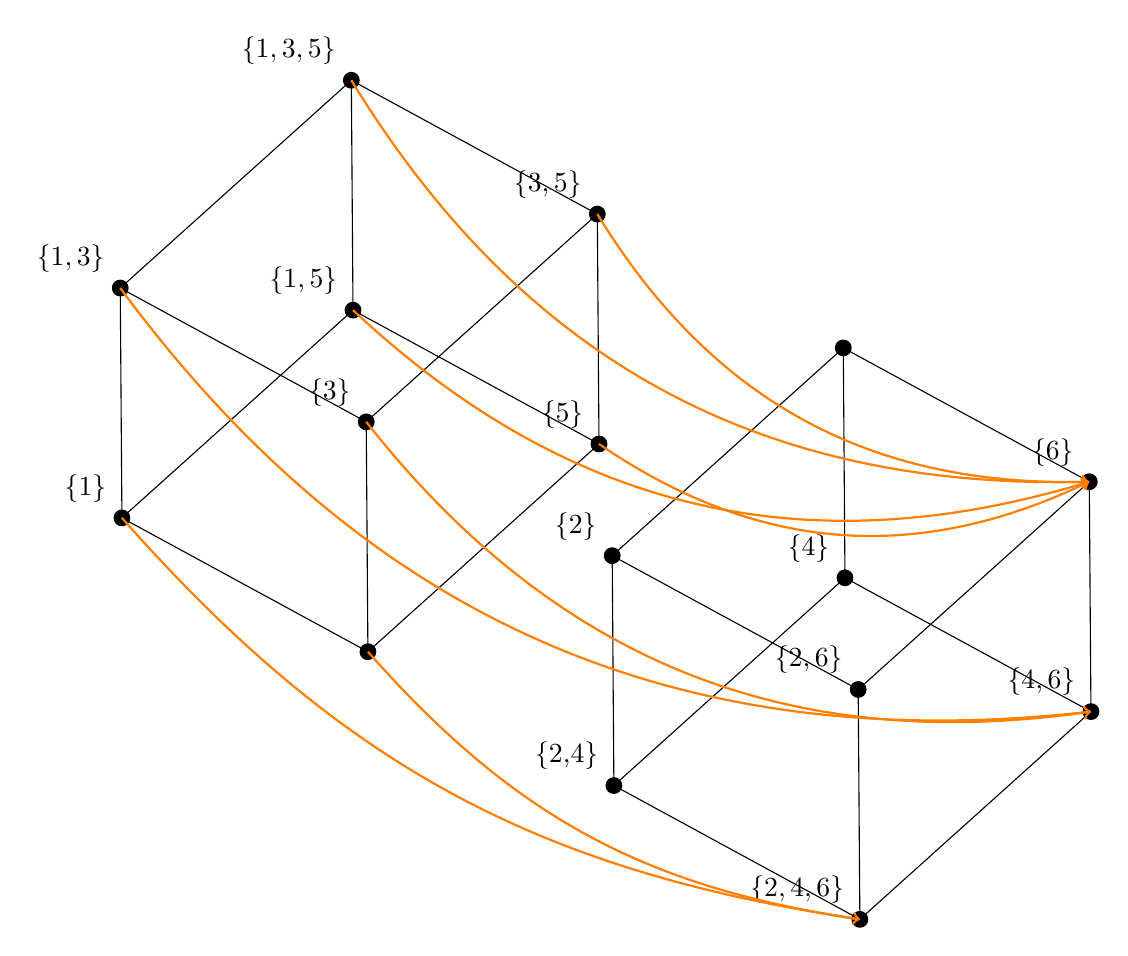
\begin{tikzpicture}[transform shape, rotate around z=-10, rotate around x=25, rotate around y=-20]

        \coordinate (A) at (0,0,0);
        \coordinate (B) at (4,0,0);
        \coordinate (C) at (4,4,0);
        \coordinate (D) at (0,4,0);
        \coordinate (E) at (0,0,4);
        \coordinate (F) at (4,0,4);
        \coordinate (G) at (4,4,4);
        \coordinate (H) at (0,4,4);

        \foreach \p/\t in { A/{$\{1,5\}$},
                            B/{$\{5\}$},
                            C/{$\{3,5\}$},
                            D/{$\{1,3,5\}$},
                            E/{\{1\}},
                            F/{$\varnothing$},
                            G/{$\{3\}$},
                            H/{$\{1,3\}$}}
            \node[draw, fill, circle, inner sep=2pt, label={135:\t}] (A\p) at (\p) {};

        \draw (A) -- (B) -- (C) -- (D) -- cycle; % Base
        \draw (E) -- (F) -- (G) -- (H) -- cycle; % Top
        \draw (A) -- (E);
        \draw (B) -- (F);
        \draw (C) -- (G);
        \draw (D) -- (H);

        \coordinate (I) at (8,0,0);
        \coordinate (J) at (12,0,0);
        \coordinate (K) at (12,4,0);
        \coordinate (L) at (8,4,0);
        \coordinate (M) at (8,0,4);
        \coordinate (N) at (12,0,4);
        \coordinate (O) at (12,4,4);
        \coordinate (P) at (8,4,4);

        \foreach \p/\t in { I/{$\{4\}$},
                            J/{$\{4,6\}$},
                            K/{$\{6\}$},
                            L/{$\varnothing$},
                            M/{\{2,4\}},
                            N/{$\{2,4,6\}$},
                            O/{$\{2,6\}$},
                            P/{$\{2\}$}}
            \node[draw, fill, circle, inner sep=2pt, label={135:\t}] (B\p) at (\p) {};

        \draw (I) -- (J) -- (K) -- (L) -- cycle; % Base
        \draw (M) -- (N) -- (O) -- (P) -- cycle; % Top
        \draw (I) -- (M);
        \draw (J) -- (N);
        \draw (K) -- (O);
        \draw (L) -- (P);

        \draw[->, color=orange, bend right=20, thick] (E) to node[above] {} (N);
        \draw[->, color=orange, bend right=20, thick] (F) to node[above] {} (N);
        \draw[->, color=orange, bend right=30, thick] (G) to node[above] {} (J);
        \draw[->, color=orange, bend right=30, thick] (H) to node[above] {} (J);
        \draw[->, color=orange, bend right=30, thick] (A) to node[above] {} (K);
        \draw[->, color=orange, bend right=30, thick] (B) to node[above] {} (K);
        \draw[->, color=orange, bend right=30, thick] (C) to node[above] {} (K);
        \draw[->, color=orange, bend right=30, thick] (D) to node[above] {} (K);
    \end{tikzpicture}
\end{figure}
L'obiettivo è costruire una funzione di concretizzazione che permetta di 
vedere l'insieme a destra come un'astrazione del dominio a sinistra.
\[
  \forall \mathcal{A}' \subseteq \mathcal{A} .
  \quad \alpha(\mathcal{A}') = \{b \in \mathcal{B} \mid \mathcal{A}' \subseteq b\}  
\]
Dove dal punto di vista formale si tratta di una funzione monotona che 
mappa un insieme nell'insieme più grande di 
elementi in cui tutti gli elementi sono più grandi dell'insieme di partenza.

Da quello che osserviamo solo tre elementi di elementi sono immagine di 
$\alpha$ secondo la definizione.

Tutti gli altri elementi sono inutili all'interno del significato di 
tale astrazione. Fatto che possiamo verificare calcolando la funzione 
$\gamma$ che è la funzione di astrazione.
\[
  \forall \mathcal{B}' \subseteq \mathcal{B} . 
    \quad \gamma(\mathcal{B}') = \{ a \in \mathcal{A} \mid a \subseteq \mathcal{B}' \}
\]
La funzione $\gamma$ preso un elemento astratto restituisce il suo significato 
concreto, in questo caso l'insieme massimale di elementi che sono più piccoli.
\begin{figure}[H]
    \centering
    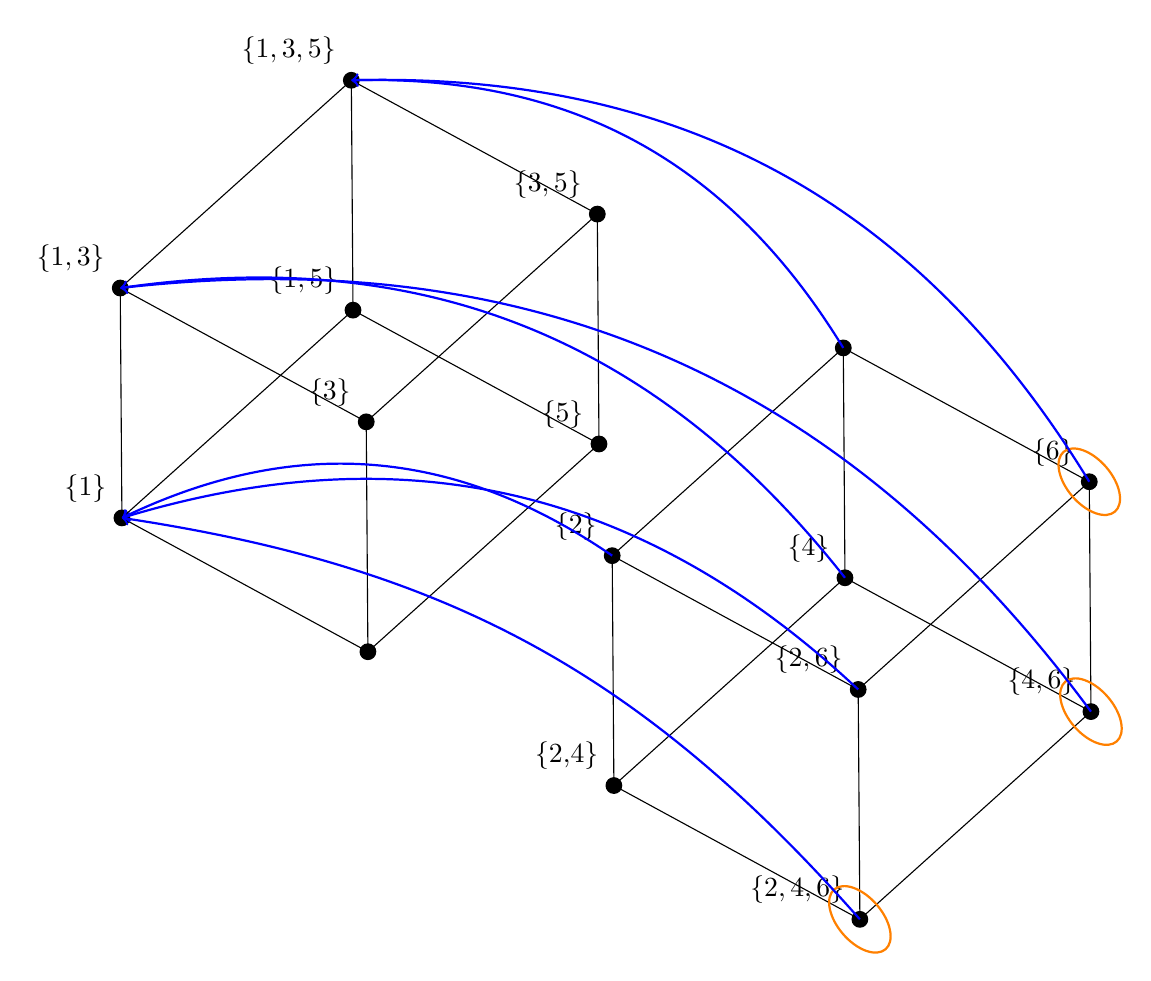
\begin{tikzpicture}[transform shape, rotate around z=-10, rotate around x=25, rotate around y=-20]

        \coordinate (A) at (0,0,0);
        \coordinate (B) at (4,0,0);
        \coordinate (C) at (4,4,0);
        \coordinate (D) at (0,4,0);
        \coordinate (E) at (0,0,4);
        \coordinate (F) at (4,0,4);
        \coordinate (G) at (4,4,4);
        \coordinate (H) at (0,4,4);

        \foreach \p/\t in { A/{$\{1,5\}$},
                            B/{$\{5\}$},
                            C/{$\{3,5\}$},
                            D/{$\{1,3,5\}$},
                            E/{\{1\}},
                            F/{$\varnothing$},
                            G/{$\{3\}$},
                            H/{$\{1,3\}$}}
            \node[draw, fill, circle, inner sep=2pt, label={135:\t}] (A\p) at (\p) {};

        \draw (A) -- (B) -- (C) -- (D) -- cycle; % Base
        \draw (E) -- (F) -- (G) -- (H) -- cycle; % Top
        \draw (A) -- (E);
        \draw (B) -- (F);
        \draw (C) -- (G);
        \draw (D) -- (H);

        \coordinate (I) at (8,0,0);
        \coordinate (J) at (12,0,0);
        \coordinate (K) at (12,4,0);
        \coordinate (L) at (8,4,0);
        \coordinate (M) at (8,0,4);
        \coordinate (N) at (12,0,4);
        \coordinate (O) at (12,4,4);
        \coordinate (P) at (8,4,4);

        \foreach \p/\t in { I/{$\{4\}$},
                            J/{$\{4,6\}$},
                            K/{$\{6\}$},
                            L/{$\varnothing$},
                            M/{\{2,4\}},
                            N/{$\{2,4,6\}$},
                            O/{$\{2,6\}$},
                            P/{$\{2\}$}}
            \node[draw, fill, circle, inner sep=2pt, label={135:\t}] (B\p) at (\p) {};

        \draw (I) -- (J) -- (K) -- (L) -- cycle; % Base
        \draw (M) -- (N) -- (O) -- (P) -- cycle; % Top
        \draw (I) -- (M);
        \draw (J) -- (N);
        \draw (K) -- (O);
        \draw (L) -- (P);

        %cerchio i punti che sono immagine di alpha
        \draw[circle, color=orange, thick] (K) circle (0.5);
        \draw[circle, color=orange, thick] (J) circle (0.5);
        \draw[circle, color=orange, thick] (N) circle (0.5);

        \draw[->, color=blue, bend right=20, thick] (N) to node[above] {} (E);
        \draw[->, color=blue, bend right=30, thick] (O) to node[above] {} (E);
        \draw[->, color=blue, bend right=30, thick] (P) to node[above] {} (E);
        \draw[->, color=blue, bend right=30, thick] (J) to node[above] {} (H);
        \draw[->, color=blue, bend right=30, thick] (I) to node[above] {} (H);
        \draw[->, color=blue, bend right=30, thick] (K) to node[above] {} (D);
        \draw[->, color=blue, bend right=30, thick] (L) to node[above] {} (D);
\end{tikzpicture}
\end{figure}
Quindi emergono 3 elementi, ovvero $\{1,3,5\}$, $\{1,3\}$ e $\{1\}$,
che sono i più concreti tra quelli che hanno la stessa 
immagine astratta, ovvero $\{4\}$, $\{4,6\}$ e $\{6\}$.

Verifichiamo che $\alpha$ e $\gamma$ rispettano le condizioni sull'essere 
connessioni di Galois.

Partendo dall'insieme vuoto e applicando $\alpha$ otteniamo l'insieme
$\{4\}$ che è l'immagine astratta di $\{ 2,4,6 \}$, applicando $\gamma$
otteniamo l'insieme $\{1\}$. Quindi
$\gamma \circ \alpha(\varnothing) \geq \varnothing$, e provandolo per tutti 
gli elementi otteniamo lo stesso risultato generico:
\[
  \gamma \circ \alpha(c) \geq c  
\]
e anche la condizione opposta:
\[
  \alpha \circ \gamma(a) \leq a
\]
Quindi $\alpha$ e $\gamma$ sono connessioni di Galois.

Per riuscire a eliminare gli elementi inutili possiamo applicare
il concetto relativo all'inserzione di Galois, quindi:
\[
  \mathcal{B}' \equiv \mathcal{B}''
  \iff \gamma(\mathcal{B}') = \gamma(\mathcal{B}'') 
  \iff \forall a \in
  \mathcal{A} . \quad a \mathcal{RB}' \iff a \mathcal{RB}'' 
\]
La differenza è che $ \alpha \circ \gamma(a) = a $, quindi
vediamo che modificando il dominio astratto e non le astrazioni 
otteniamo un'inserzione di Galois, osserviamo quindi gli elementi che 
hanno lo stesso significato.
quindi:
\begin{itemize}
    \item $\varnothing$ e $\{6\}$ hanno lo stesso significato, quindi
    vengono mappati in un unico elemento, che è $\{6\}$;
    \item $\{4\}$ e $\{4,6\}$ hanno lo stesso significato, quindi
    vengono mappati in un unico elemento, che è $\{4,6\}$;
    \item $\{2,4\}$, $\{2,4,6\}$, $\{2,6\}$ e $\{2\}$ hanno lo stesso
    significato e vengono mappati in un unico elemento, che è $\{2,4,6\}$.
\end{itemize} 
Accorpando gli elementi astratti che hanno lo stesso significato.
Quindi otteniamo il seguente diagramma:
\begin{figure}[H]
    \centering
    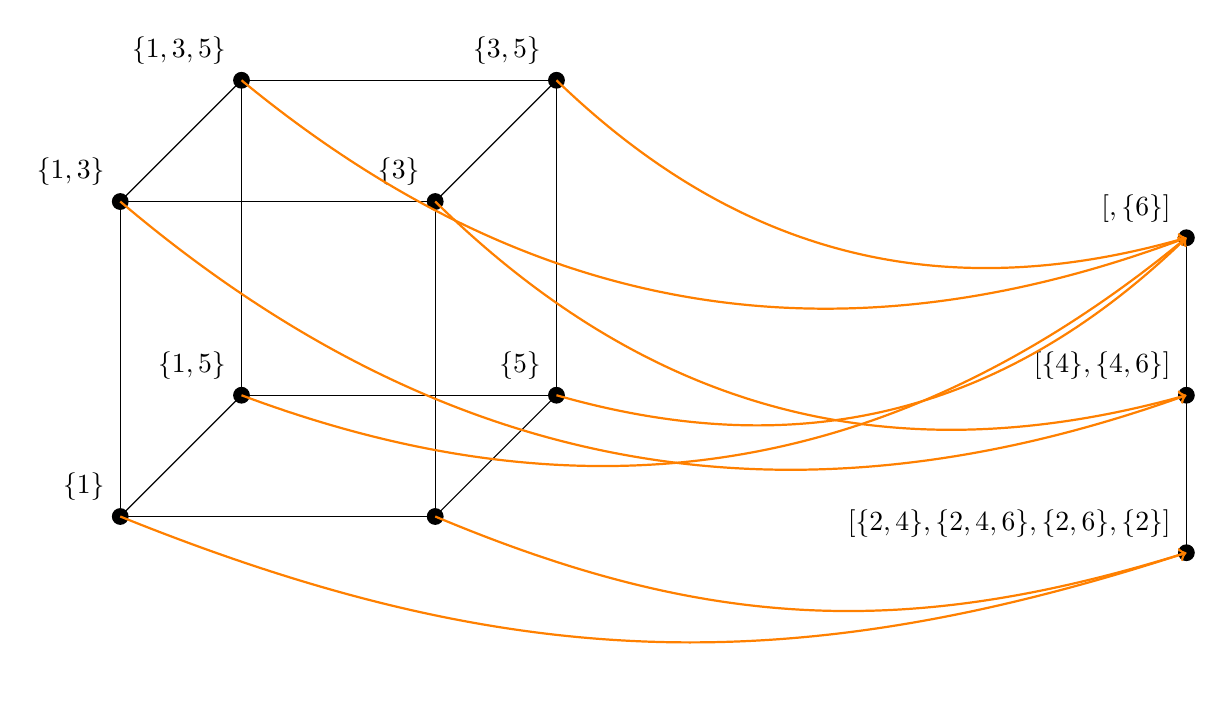
\begin{tikzpicture}[transform shape]

        \coordinate (A) at (0,0,0);
        \coordinate (B) at (4,0,0);
        \coordinate (C) at (4,4,0);
        \coordinate (D) at (0,4,0);
        \coordinate (E) at (0,0,4);
        \coordinate (F) at (4,0,4);
        \coordinate (G) at (4,4,4);
        \coordinate (H) at (0,4,4);

        \foreach \p/\t in { A/{$\{1,5\}$},
                            B/{$\{5\}$},
                            C/{$\{3,5\}$},
                            D/{$\{1,3,5\}$},
                            E/{\{1\}},
                            F/{$\varnothing$},
                            G/{$\{3\}$},
                            H/{$\{1,3\}$}}
            \node[draw, fill, circle, inner sep=2pt, label={135:\t}] (A\p) at (\p) {};

        \draw (A) -- (B) -- (C) -- (D) -- cycle; % Base
        \draw (E) -- (F) -- (G) -- (H) -- cycle; % Top
        \draw (A) -- (E);
        \draw (B) -- (F);
        \draw (C) -- (G);
        \draw (D) -- (H);

        %retta 
        \coordinate (J) at (12,0,0);
        \coordinate (K) at (12,2,0);
        \coordinate (N) at (12,-2,0);

        %connetto i punti
        \draw (J) -- (K) -- (N); 


        \foreach \p/\t in { J/{$[\{4\},\{4,6\}]$},
                            K/{$[\varnothing,\{6\}]$},
                            N/{$[\{2,4\},\{2,4,6\},\{2,6\},\{2\}]$}}
            \node[draw, fill, circle, inner sep=2pt, label={135:\t}] (B\p) at (\p) {};

            \draw[->, color=orange, bend right=20, thick] (E) to node[above] {} (N);
            \draw[->, color=orange, bend right=20, thick] (F) to node[above] {} (N);
            \draw[->, color=orange, bend right=30, thick] (G) to node[above] {} (J);
            \draw[->, color=orange, bend right=30, thick] (H) to node[above] {} (J);
            \draw[->, color=orange, bend right=30, thick] (A) to node[above] {} (K);
            \draw[->, color=orange, bend right=30, thick] (B) to node[above] {} (K);
            \draw[->, color=orange, bend right=30, thick] (C) to node[above] {} (K);
            \draw[->, color=orange, bend right=30, thick] (D) to node[above] {} (K);
\end{tikzpicture}
\end{figure}
Definiamo quindi una relazione di equivalenza tale per cui, se prendiamo 
anziché gli elementi astratti, le classi di equivalenza rispetto a tale relazione,
otteniamo un'inserzione di Galois, senza variare le funzioni 
$\alpha$ e $\gamma$, riducendo il dominio astratto.

Vediamo come questi formalismi (\textit{in particolare l'inserzione di
Galois}) sono equivalenti ad altri due formalismi, che però spostano 
l'osservazione dal dominio astratto, ovvero $\mathcal{A}$,
che ha una propria rappresentazione, a quello del dominio degli oggetti 
concreti che vogliamo osservare. Invece di guardare un mondo astratto 
rappresentato in un modo diverso, osserviamo il loro significato sul 
mondo concreto. Specifichiamo gli oggetti che osserviamo con precisione, ma 
nel mondo concreto e quindi modello con una funzione, chiamata \textbf{
funzione di chiusura superiore}, o un sottodominio, chiamato 
\textbf{Moore family}, ovvero l'astrazione del dominio concreto.

\section{Operatore di chiusura superiore (\texttt{UCO})}
Introduciamo questo nuovo concetto, che è una tipologia di funzioni che possiamo 
definire su un dominio. Supponiamo di avere un dominio $\mathcal{P}$ con un suo 
ordinamento $\leq_\mathcal{P}$ (\textit{in generale su reticoli completi}).

Allora una funzione $\rho : \mathcal{P} \to \mathcal{P}$ è un \texttt{UCO} 
se la funzione $\rho$ è:
\begin{itemize}
    \item \textbf{Monotona}: $\forall x,y \in \mathcal{P} \quad x \leq_\mathcal{P} y \implies \rho(x) \leq_\mathcal{P} \rho(y)$;
    \item \textbf{Estensiva}: $\forall x \in \mathcal{P} \quad x \leq_\mathcal{P} \rho(x)$;
    \item \textbf{Idempotente}: $\forall x \in \mathcal{P} \quad \rho(\rho(x)) = \rho(x)$.
\end{itemize}
Ovvero che $\rho$ può perdere informazione, ma tale informazione viene persa 
tutta in un'unica applicazione, ogni successiva applicazione non aggiunge
ulteriore imprecisione.

\begin{tcolorbox}[title = $\gamma \circ \alpha$ è un \texttt{UCO} nelle connessioni di Galois]
Questo perché sappiamo che $\gamma \circ \alpha$ è monotona, poiché 
si tratta di composizione di funzioni monotone, è estensiva perché
nelle proprietà delle connessioni di Galois abbiamo che 
$\gamma \circ \alpha(c) \geq c$ ed è idempotente, ovvero
perché $\gamma \circ \alpha \circ \gamma \circ \alpha(c) = 
\gamma \circ \texttt{id} \circ \alpha(c) = \gamma \circ \alpha(c)$, poiché 
$\gamma \circ \alpha \equiv \texttt{id}$.  
\end{tcolorbox}
\subsection{Esempio di \texttt{UCO}}
\begin{figure}[H]
    \centering
    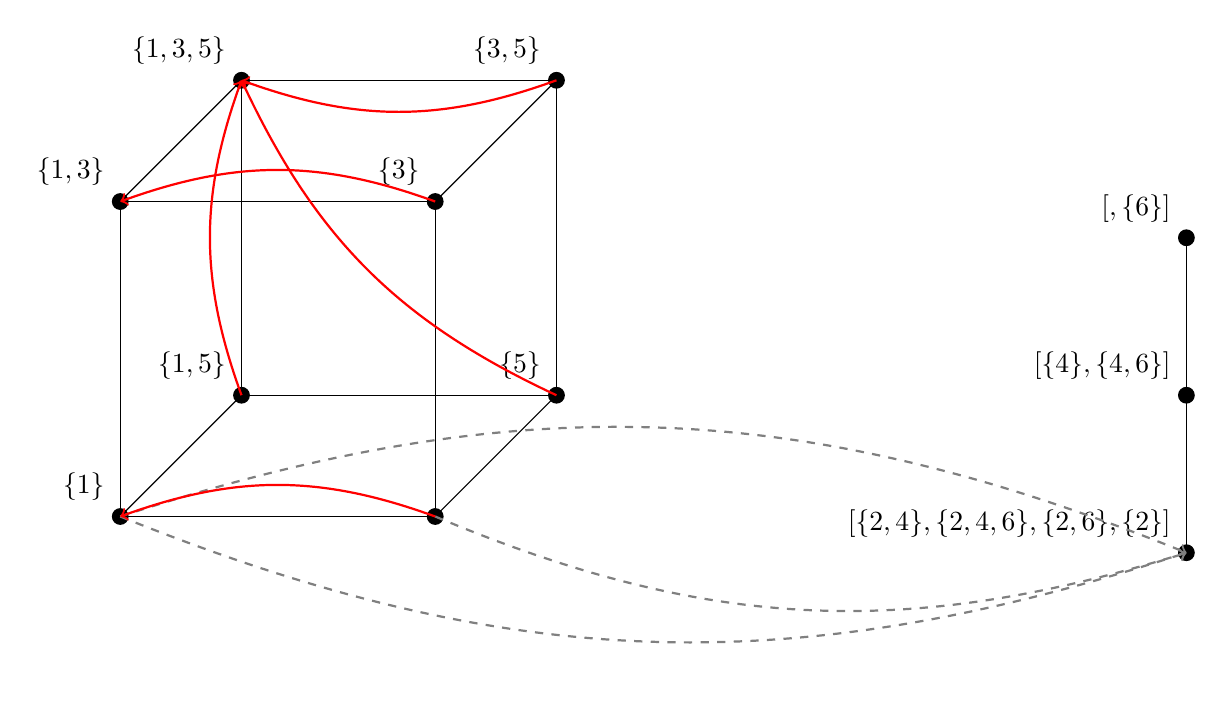
\begin{tikzpicture}[transform shape]

        \coordinate (A) at (0,0,0);
        \coordinate (B) at (4,0,0);
        \coordinate (C) at (4,4,0);
        \coordinate (D) at (0,4,0);
        \coordinate (E) at (0,0,4);
        \coordinate (F) at (4,0,4);
        \coordinate (G) at (4,4,4);
        \coordinate (H) at (0,4,4);

        \foreach \p/\t in { A/{$\{1,5\}$},
                            B/{$\{5\}$},
                            C/{$\{3,5\}$},
                            D/{$\{1,3,5\}$},
                            E/{\{1\}},
                            F/{$\varnothing$},
                            G/{$\{3\}$},
                            H/{$\{1,3\}$}}
            \node[draw, fill, circle, inner sep=2pt, label={135:\t}] (A\p) at (\p) {};

        \draw (A) -- (B) -- (C) -- (D) -- cycle; % Base
        \draw (E) -- (F) -- (G) -- (H) -- cycle; % Top
        \draw (A) -- (E);
        \draw (B) -- (F);
        \draw (C) -- (G);
        \draw (D) -- (H);

        %retta 
        \coordinate (J) at (12,0,0);
        \coordinate (K) at (12,2,0);
        \coordinate (N) at (12,-2,0);

        %connetto i punti
        \draw (J) -- (K) -- (N); 


        \foreach \p/\t in { J/{$[\{4\},\{4,6\}]$},
                            K/{$[\varnothing,\{6\}]$},
                            N/{$[\{2,4\},\{2,4,6\},\{2,6\},\{2\}]$}}
            \node[draw, fill, circle, inner sep=2pt, label={135:\t}] (B\p) at (\p) {};

            \draw[->, color=gray, bend right=20, thick, dashed] (E) to node[above] {} (N);
            \draw[->, color=gray, bend right=20, thick, dashed] (F) to node[above] {} (N);
            \draw[->, color=gray, bend left=20, thick, dashed] (E) to node[above] {} (N);
            % Disegna la freccia che va su se stessa
            \draw[->, color=red, bend right=20, thick, red] (F) to node[above] {} (E);
            \draw[->, color=red, bend right=20, thick, red] (G) to node[above] {} (H);
            \draw[->, color=red, bend left=20, thick, red] (A) to node[above] {} (D);
            \draw[->, color=red, bend left=20, thick, red] (B) to node[above] {} (D);
            \draw[->, color=red, bend left=20, thick, red] (C) to node[above] {} (D);


\end{tikzpicture}
\end{figure}
\[
    \gamma \circ \alpha (\mathcal{A}') = 
    \gamma (\{b \in \mathcal{B} \mid \mathcal{A}' \mathcal{R} b\}) = 
    \{ a \in \mathcal{A} \mid a \mathcal{R} \{ b \in \mathcal{R} b\}\}
    = \{a \in \mathcal{A} \mid  \forall b \in \mathcal{B} . \mathcal{A}'
    \mathcal{R} b \implies a \mathcal{R} b\}
\]
Se partiamo dall'insieme vuoto $\varnothing$ e applichiamo $\gamma \circ \alpha$
otteniamo l'insieme $\{1\}$, se applichiamo nuovamente $\gamma \circ \alpha$ 
otteniamo l'insieme $\{1\}$, ovvero l'insieme di partenza. Quindi è \textbf{idempotente},
e tale risultato è l'\texttt{UCO}.

L'\texttt{UCO} che definiamo sul dominio concreto permette di associare ad ogni elemento concreto l'osservazione 
precisa che abbiamo scelto di guardare e che meglio approssima l'oggetto da cui siamo partiti.

Le immagini del nostro \texttt{UCO}, che sono i punti fissi, sono i significati degli oggetti astratti, ovvero 
gli elementi concreti che abbiamo scelto di osservare con precisione, ed è da qui che cerchiamo di 
approssimare gli altri elementi.

I punti in questione sono quindi i significati degli oggetti astratti, ovvero esattamente gli
elementi concreti che
abbiamo deciso di osservare con precisione. Gli elementi in cui cercare l'approssimazione di tutti 
gli altri elementi concreti.
\begin{tcolorbox}
    L'\texttt{UCO} altro non fa che associare ad ogni elemento concreto la sua migliore 
    approssimazione. Possiamo ignorare la rappresentazione astratta degli elementi 
    che abbiamo scelto di osservare con precisione e consideriamo solamente 
    la trasformazione che associa ad ogni elemento concreto la sua migliore approssimazione,
    ovvero che associa ad ogni elemento concreto la proprietà astratta di interesse che lo 
    caratterizza.
\end{tcolorbox}
Ciò che ci permette di fare il passaggio agli operatori di chiusura superiore è di 
dimenticarci del dominio astratto.
\begin{figure}[H]
    \centering
    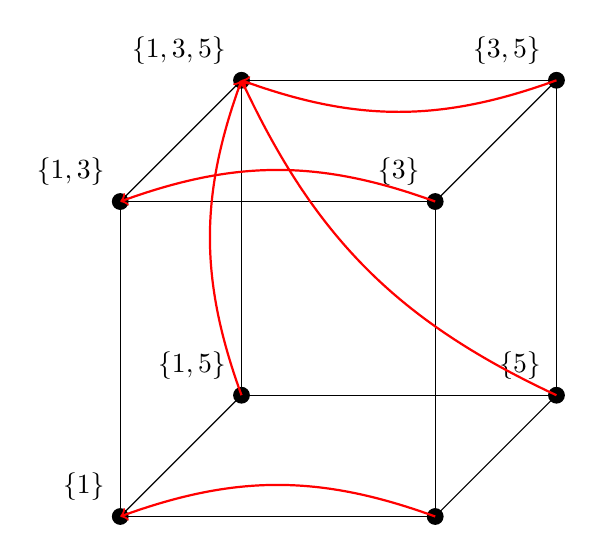
\begin{tikzpicture}[transform shape]

        \coordinate (A) at (0,0,0);
        \coordinate (B) at (4,0,0);
        \coordinate (C) at (4,4,0);
        \coordinate (D) at (0,4,0);
        \coordinate (E) at (0,0,4);
        \coordinate (F) at (4,0,4);
        \coordinate (G) at (4,4,4);
        \coordinate (H) at (0,4,4);

        \foreach \p/\t in { A/{$\{1,5\}$},
                            B/{$\{5\}$},
                            C/{$\{3,5\}$},
                            D/{$\{1,3,5\}$},
                            E/{\{1\}},
                            F/{$\varnothing$},
                            G/{$\{3\}$},
                            H/{$\{1,3\}$}}
            \node[draw, fill, circle, inner sep=2pt, label={135:\t}] (A\p) at (\p) {};

        \draw (A) -- (B) -- (C) -- (D) -- cycle; % Base
        \draw (E) -- (F) -- (G) -- (H) -- cycle; % Top
        \draw (A) -- (E);
        \draw (B) -- (F);
        \draw (C) -- (G);
        \draw (D) -- (H);

        \draw[->, color=red, bend right=20, thick, red] (F) to node[above] {} (E);
        \draw[->, color=red, bend right=20, thick, red] (G) to node[above] {} (H);
        \draw[->, color=red, bend left=20, thick, red] (A) to node[above] {} (D);
        \draw[->, color=red, bend left=20, thick, red] (B) to node[above] {} (D);
        \draw[->, color=red, bend left=20, thick, red] (C) to node[above] {} (D);
\end{tikzpicture}
\end{figure}
\section{Moore family}
Siano $\mathcal{P}, \leq_\mathcal{P}$ un reticolo completo, allora
$x \subseteq \mathcal{P}$ è un \textbf{insieme di Moore} se 
$x = \mathcal{M}(x)$, ovvero \textbf{chiusura di Moore di x}.
dove:
\[
  \mathcal{M}(x) =  \biggl\{\bigwedge_\mathcal{P} \mathcal{S} \mid \mathcal{S} \subseteq x\biggr\}
\]
Dove $x$ è chiuso per $\bigwedge_\mathcal{P}$, ovvero per ogni sottoinsieme $\mathcal{S} \subseteq x$.

In altri termini:
\[
  Sia \qquad \mathcal{S} \subseteq x \implies \bigwedge_\mathcal{P} \mathcal{S} \in x  
\]

\begin{figure}[H]
    \centering
    \begin{tikzpicture}[transform shape]

        \coordinate (A) at (0,0,0);
        \coordinate (B) at (4,0,0);
        \coordinate (C) at (4,4,0);
        \coordinate (D) at (0,4,0);
        \coordinate (E) at (0,0,4);
        \coordinate (F) at (4,0,4);
        \coordinate (G) at (4,4,4);
        \coordinate (H) at (0,4,4);

        
        \node[draw, fill, circle, inner sep=2pt, label={135:$0^+$}] (q) at (H) {};
        \node[draw, fill, circle, inner sep=2pt, label={135:$0^-$}] (r) at (C) {};
        \node[draw, fill, circle, inner sep=2pt, label={135:$\mathbb{Z}$}] (u) at (D) {};
        \node[draw, fill, circle, inner sep=2pt, label={135:$\varnothing$}] (t) at (F) {};

        \draw (A) -- (B) -- (C) -- (D) -- cycle; % Base
        \draw (E) -- (F) -- (G);
        \draw[red] (G) -- (H);
        \draw (H) -- (E);
        \draw (A) -- (E);
        \draw (B) -- (F);
        \draw[red] (C) -- (G);
        \draw (D) -- (H);

\end{tikzpicture}
\end{figure}
Considerando il sottoreticolo di $\wp(\mathcal{Z})$ e prendendo come elementi di x: $0^+, 0^-,
\mathbb{Z}, \varnothing$;  allora $x$ non è Moore family di $\wp(\mathcal{Z})$, perché prendendo
la congiunzione logica \texttt{AND} tra due elementi di $0^+$ e  $0^-$ otteniamo un elemento che 
non appartiene a $x$ (\textit{tale elemento è lo zero}).
\[
  \exists \mathcal{S} = \{ 0^+, 0^- \} \, t.c. \, \bigwedge_\mathcal{P} \mathcal{S} = 0 \notin x
\]
Nella nostra concezione di dominio astratto, l'insieme dei punti fissi di un \texttt{UCO} 
$\rho:  \mathcal{P} \to \mathcal{P}$ formano una Moore family di $\mathcal{P}$. Di fatto ogni Moore family di un 
dominio concreto rappresenta una proprietà di un dominio astratto.

\begin{tcolorbox}
    I punti fissi di $\rho$ sono una Moore family del dominio concreto, ovvero di $\wp(\mathcal{A})$.
\end{tcolorbox}
\subsection{Considerazioni}
Disponiamo di tre modi differenti per rappresentare un dominio astratto:
\begin{itemize}
    \item \textbf{UCO}: $\rho: \mathcal{P} \to \mathcal{P}$;
    \item \textbf{Moore family}: $x \subseteq \mathcal{P}$;
    \item \textbf{Inserzioni di Galois}: $(\mathcal{C}, \leq_\mathcal{C}) \galoiS{\alpha}{\gamma}
    (\mathcal{A}, \leq_\mathcal{A})$.
\end{itemize}
Ha senso parlare delle tre rappresentazioni, perché ognuno può essere utilizzato in contesti diversi.
Le connessioni di Galois sono utili per rappresentare dominio astratto, quindi dipende dalla rappresentazione degli elementi, 
ed è utile durante l'implementazione, in modo da rappresentare in modo semplice le proprietà 
di oggetti astratti.

Gli altri due metodi di modellazione del dominio astratto sul dominio concreto sono indipendenti 
dalla rappresentazione di elementi perché si parla di elementi astratti attraverso i loro significati, 
indipendenti dall'astrazione. Chiaramente meno adatti ai contesti applicativi, ma più adatti 
in contesti di verifica di proprietà sui domini astratti, o comunque ragionamenti formali sulle 
caratteristiche del dominio astratto e dell'analisi.

Quindi in base al contesto si decide la metodologia di rappresentazione adatta.

\subsection{Relazione tra Moore family e inserzioni di Galois}
\begin{itemize}
    \item Supponiamo di partire da un'inserzione di Galois.
    \[
        \mathcal{C} \galoiS{\alpha}{\gamma} \mathcal{A} \iff \mathcal{A} \textit{ è isomorfo a una famiglia di 
        Moore di } \mathcal{C}
    \]
    Quindi
    \[
      \exists \mathcal{X} \textit{famiglia di Moore di } \mathcal{C} \, t.c. \, 
      \exists \iota : \mathcal{A} \rightarrow \mathcal{X}
    \]
    Esiste quindi una funzione biunivoca tra $\mathcal{A}$ e $\mathcal{X}$.
    \item Supponiamo di partire da un \texttt{UCO}.
    \[
        \rho \in \texttt{UCO}(\mathcal{C}) \implies \exists \, \textit{isomorfismo tra }
        \iota: \rho(\mathcal{C}) \to \mathcal{A}
    \]
    Dove $\mathcal{A}$ e una qualunque rappresentazione degli elementi di $\rho(\mathcal{C})$.
    
    Quindi $\mathcal{C} \galoiS{\iota^{-1}}{  \iota\,\circ\,\rho} \mathcal{A}$.
\end{itemize}
\begin{tcolorbox}
    \[
        \iota^{-1} \, \circ \, \iota \, \circ \, \rho = \rho
    \]
    Questo perché $\iota^{-1} \, \circ \, \iota = \texttt{id}$ e $\iota \, \circ \, \rho = \alpha$.

    \[
        \iota \, \circ \, \rho \, \circ \, \iota^{-1}(\alpha) 
        = \iota \, \circ \, \rho \, \circ \, \rho(\alpha) 
        = \iota \, \circ \, \rho(\alpha)  = \alpha
    \]
    Dove $\iota^{-1}(\alpha) \in \rho$
\end{tcolorbox}
\subsection{Relazione tra inserzioni di Galois e \texttt{UCO}}
La relazione è immediata, poiché se $\mathcal{C} \galoiS{\alpha}{\gamma} \mathcal{A}$, allora 
$\gamma \, \circ \, \alpha \in \texttt{UCO}$
\subsection{Relazione tra \texttt{UCO} e Moore family}
La relazione è immediata, poiché se $\rho \in \texttt{UCO}(\mathcal{C})$, allora $\rho(\mathcal{C})$, che 
è l'insieme dei punti fissi è famiglia di Moore di $\mathcal{C}$.
\section{Reticolo delle interpretazioni astratte}
Supponiamo di avere un reticolo completo
\[
    \langle \mathcal{C}, \leq_\mathcal{P}, \land, \lor, \top, \bot \rangle
\]
Abbiamo inoltre l'insieme di tutti i domini astratti $\mathcal{A}_i \in \texttt{UCO}(\mathcal{C})$.
\[
    \langle \texttt{UCO}(\mathcal{C}), \sqsubseteq, \sqcap, \sqcup, \lambda x . \top,
    \lambda x . x \rangle
\] 
\texttt{UCO} ordinato per precisione relativa è un reticolo completo. 

L'ordinamento di precisione relativa permette di confrontare il grado di precisione dei domini 
astratti, dove un elemento è più preciso se contiene più elementi. 
\[
  \mathcal{A}_1 \sqsubseteq \mathcal{A}_2 \iff \mathcal{A}_1 \textit{ corrisponde ad un insieme 
  di elementi più grande} 
\]
\[
    \rho \sqsubseteq \eta \iff \forall y \in \mathcal{C} \, . \, \rho(y) \leq \eta(y)
    \iff \rho(\mathcal{C}) \subseteq \eta(\mathcal{C})
\]
Con questo ordinamento relativo possiamo definire un operatore di greatest lower bound, 
chiamato prodotto ridotto, $\sqcap \mathcal{A}_i$. Viene preso il più piccolo dominio astratto tra 
tutti i domini che contengono $\mathcal{A}_i$. Ricordiamo che non è banalmente l'unione, l'unione 
può non essere una {Moore family}.

L'operatore di least upper bound, chiamato prodotto esteso, $\sqcup \mathcal{A}_i$.
Viene preso il più grande dominio astratto contenuto in tutti i domini astratti.
Quindi:
\[
    \bigcap \mathcal{A}_i = \sqcap \mathcal{A}_i
\]

L'operatore $\lambda x . \top$ è il dominio astratto più astratto, ovvero quello che 
non osserva nulla, tutti gli elementi concreti sono mappati nel top.

L'operatore $\lambda x . x$ è il dominio astratto più concreto, ovvero quello che
osserva tutto, tutti gli elementi concreti sono mappati in se stessi, quindi l'identità.
\section{Computazioni astratte}
La computazione astratta tratta di come si trasferisce un calcolo dal dominio concreto al
dominio astratto.
L'obiettivo è quello di trasferire il calcolo, partiamo da una funzione definita su
oggetti concreti: $f : c \to c$, che sono le nostre operazioni su elementi di $\mathcal{C}$, 
che vogliamo trasferire in operazioni su elementi di $\mathcal{A}$: $f^\# : a \to a$.

Diciamo che $f^\#$ è corretta per $f$ se $\alpha \, \circ \,
f(c) \leq_\mathcal{A} f^\# \, \circ \, \alpha(c)$.

\begin{figure}[H]
    \centering
    \begin{tikzpicture}[>=stealth, node distance=2cm]

        % Define styles
        \tikzstyle{set} = [ellipse, draw, minimum height=4cm, minimum width=6cm, align=center]
        \tikzstyle{arrow} = [->, thick];
    
        % Nodes
        \node[set] (C) at (0,0) {$C$};
        \node[set, right=of C] (A) {$A$};
        
        
        \node[circle, draw, fill=black, inner sep=2pt, label=below:$c$] (pointC) at (1,-1) {};
        \node[circle, draw, fill=black, inner sep=2pt, label=below:$\alpha(c)$] (pointAlphaC) at (7,-1) {};
        \draw[arrow, orange] (pointC) to [bend left =] (pointAlphaC);
        \node[circle, draw, fill=black, inner sep=2pt] (pointA) at (8,1) {};
        \draw[->, thick] (pointAlphaC) to [bend right] (pointA);

        \node[circle, draw, fill=black, inner sep=2pt] (result) at (7,0) {};

        \node[circle, draw, fill=black, inner sep=2pt]
        (pointGammaA) at (1,0) {};
        \draw[arrow, green] (pointGammaA) to [bend left] (result);
        \draw[->, thick] (pointC) to [bend left] (pointGammaA);

        % Scrivo alpha sopra la freccia
        \node at (4,0.2) {$\alpha$};
        \node at (4,1.2) {$\alpha$};
        \node at (0.5,-0.5) {$f$};
        \node at (8,-0.7) {$f^\#$};

        % segmento tra result e pointA
        \draw[-, thick, blue] (result) to (pointA);
        
    \end{tikzpicture}
\end{figure}
Il calcolo astratto può perdere informazione rispetto alla proprietà del calcolo concreto. Il 
calcolo astratto è corretto se approssima la proprietà del calcolo concreto. In modo analogo 
possiamo caratterizzare la correttezza confrontato i risultati sul mondo concreto.

\begin{figure}[H]
    \centering
    \begin{tikzpicture}[>=stealth, node distance=2cm]

        % Define styles
        \tikzstyle{set} = [ellipse, draw, minimum height=4cm, minimum width=6cm, align=center]
        \tikzstyle{arrow} = [->, thick];
    
        % Nodes
        \node[set] (C) at (0,0) {$A$};
        \node[set, right=of C] (A) {$C$};
        
        
        \node[circle, draw, fill=black, inner sep=2pt, label=below:$a$] (pointC) at (1,-1) {};
        \node[circle, draw, fill=black, inner sep=2pt, label=below:$\gamma(a)$] (pointAlphaC) at (7,-1) {};
        \draw[arrow, orange] (pointC) to [bend left =] (pointAlphaC);
        \node[circle, draw, fill=black, inner sep=2pt] (pointA) at (8,1) {};
        \draw[->, thick] (pointAlphaC) to [bend right] (pointA);

        \node[circle, draw, fill=black, inner sep=2pt] (result) at (7,0) {};

        \node[circle, draw, fill=black, inner sep=2pt]
        (pointGammaA) at (1,0) {};
        \draw[arrow, green] (pointGammaA) to [bend left] (result);
        \draw[->, thick] (pointC) to [bend left] (pointGammaA);

        % Scrivo alpha sopra la freccia
        \node at (4,0.2) {$\gamma$};
        \node at (4,1.2) {$\gamma$};
        \node at (0.5,-0.5) {$f^\#$};
        \node at (8,-0.7) {$f$};

        % segmento tra result e pointA
        \draw[-, thick, blue] (result) to (pointA);
        
    \end{tikzpicture}
\end{figure}
Il significato del risultato del calcolo astratto approssima il risultato concreto.
Quindi $f \circ \gamma(a) \leq_\mathcal{C} \gamma \circ f^\#(a)$.

\begin{tcolorbox}
    Dato $\galois{\alpha}{\gamma} \mathcal{A}, f: c \to c$, allora $f^\# : a \to a$ 
    soddisfa la relazione  
    \[\alpha \, \circ \, f(c) \leq_\mathcal{A} f^\# \, \circ \, \alpha(c)\]
    se e solo se soddisfa
    \[f \, \circ \, \gamma(a) \leq_\mathcal{C} \gamma \, \circ \, f^\#(a)\]
\end{tcolorbox}
In particolare se partiamo dalla condizione che per ogni $x$ appartenente al dominio concreto,
$\alpha \, \circ \, f(x) \leq_\mathcal{A} f^\# \, \circ \, \alpha(x) \iff 
\alpha \, \circ \, f \, \circ \, \gamma(x) \leq_\mathcal{A} f^\#(x)$.
dove $\alpha \, \circ \, f \, \circ \, \gamma(x)$ è la funzione \textbf{best 
correct approximation}.
\[
  f^\# \textit{ è sound } \iff \textit{ approssima } f^\# \equiv \alpha \, \circ \, f \, \circ \, \gamma 
  : \mathcal{A} \to \mathcal{A}
\]
Tale costruzione va bene per gli operatori, ma non è accettabile come trasferimento per l'intera 
semantica, perché il nostro obiettivo è non passare da $f$.
\subsection{Soundness sulle chiusure}
$\alpha f(x) \leq_\mathcal{A} \alpha \circ f \circ \alpha(x)$ per monotonia di $\gamma$ 
otteniamo $\gamma \circ \alpha \circ f(x) \leq_\mathcal{C} \gamma \circ \alpha
\circ f \circ \gamma \circ \alpha(x)$. Osserviamo che abbiamo sempre $\gamma \circ \alpha$
e questo possiamo ridefinirlo come $\rho \in \texttt{UCO}$ perché abbiamo già detto che  
$\gamma \circ \alpha$ è \texttt{UCO} del dominio concreto. 

Quindi la relazione di correttezza ottenuta confrontato i due calcoli nel mondo 
astratto si riscrive in termini di chiusure esattamente in questo modo:
\[
    \rho \circ f(x) \leq_\mathcal{C} \rho \circ f \circ \rho(x)
\]

Considerando $f \, \circ \, \gamma(a) \leq_\mathcal{C} \gamma \, \circ \, f^\#(a)$, allora
$f \circ \gamma(a) \leq \gamma \circ \alpha \circ f \circ \gamma(a)$. Essendo $\gamma, \alpha$ 
connessioni di Galois, allora ogni elemento astratto è l'astrazione di un elemento concreto, 
$a = \alpha(c)$, quindi:$f \circ \gamma \circ \alpha(c) \leq \gamma
\circ \alpha \circ f \circ \gamma \circ \alpha(c)$

Otteniamo quindi:
\[
  f \circ \rho(c) \leq_\mathcal{C} \rho \circ f \circ \rho(c)
\]
La relazione è leggermente diversa, ma è equivalente. 

\begin{tcolorbox}
    Ragionare con le inserzioni di Galois garantisce per costruzione la correttezza.
    Le analisi costruite nel contesto di interpretazione astratta sono dette 
    corrette per costruzione.
\end{tcolorbox}
\subsection{Completeness sulle chiusure}
\subsubsection{Backward completeness - Relazione di precisione sul dominio $\mathcal{A}$}
Un'analisi è precisa quando eseguire il calcolo nel mondo astratto ed eseguirlo nel mondo concreto 
non fa differenza. L'informazione scartata durante la costruzione del mondo astratto, non era informazione utile per il calcolo 
che interessa effettuare. Quello che non osserviamo non è rilevante 
per il calcolo che vogliamo effettuare.
\begin{figure}[H]
    \centering
    \begin{tikzpicture}[>=stealth, node distance=2cm]

        % Define styles
        \tikzstyle{set} = [ellipse, draw, minimum height=4cm, minimum width=6cm, align=center]
        \tikzstyle{arrow} = [->, thick];
    
        % Nodes
        \node[set] (C) at (0,0) {$C$};
        \node[set, right=of C] (A) {$A$};
        
        
        \node[circle, draw, fill=black, inner sep=2pt, label=below:$c$] (pointC) at (1,-1) {};
        \node[circle, draw, fill=black, inner sep=2pt, label=below:$\alpha(c)$] (pointAlphaC) at (7,-1) {};
        \draw[arrow, orange] (pointC) to [bend left =] (pointAlphaC);
        \node[circle, draw, fill=black, inner sep=2pt] (pointA) at (7,0) {};
        \draw[->, thick] (pointAlphaC) to [bend right] (pointA);
        \node[circle, draw, fill=black, inner sep=2pt]
        (pointGammaA) at (1,0) {};
        \draw[arrow, green] (pointGammaA) to [bend left] (pointA);
        \draw[->, thick] (pointC) to [bend left] (pointGammaA);

        % Scrivo alpha sopra la freccia
        \node at (4,0.2) {$\alpha$};
        \node at (4,1.2) {$\alpha$};
        \node at (0.5,-0.5) {$f$};
        \node at (7.5,-0.5) {$f^\#$};
    \end{tikzpicture}
\end{figure}
\[
    \alpha \circ f(x) = f^\# \circ \alpha(x) 
\]
Se sostituiamo $f^\#$ con la \texttt{BCA} otteniamo:
\[
    \alpha \circ f(x) = \alpha \circ f \circ \gamma \circ \alpha(x)
\]
Possiamo applicare $\gamma$ a sinistra e a destra:
\[
    \gamma \circ \alpha \circ f(x) = \gamma \circ \alpha \circ f \circ \gamma \circ \alpha(x)
\]
Quindi
\[
    \rho \circ f(x) = \rho \circ f \circ \rho(x)
\]
La proprietà del risultato ottenuto calcolando sugli elementi astratti è la stessa 
del risultato ottenuto calcolando sugli elementi concreti. Astrarre l'input non genera nessuna 
approssimazione.
\subsubsection{Forward completeness - Relazione di precisione sul dominio $\mathcal{C}$}
Il significato del calcolo astratto coincide con il calcolo concreto; eseguendo le operazioni 
precedenti:
\[
    f^\# = \alpha \circ f \circ \gamma \qquad f \circ \rho(x) = \rho \circ f \circ \rho(x)
\]
Approssimare il risultato del calcolo astratto non genera imprecisione.
\subsubsection{Esempio di backward completeness}
Supponiamo che $\mathcal{C} = \wp(\mathcal{Z})$, $\mathcal{A} = Segni$ ($\texttt{Pos}, \texttt{Neg},
\bot, \top$) e che $f=+$.

Allora $f \rho \circ f \circ \rho \to \texttt{Pos} +^\# \texttt{Neg} = ?$ ed è evidente che abbiamo perso informazione.

Se invece facciamo il calcolo completo allora $\rho \circ f \to \texttt{Segni}(5 + (-7)) = \texttt{Neg}$, quindi 
è evidente che non siamo regolari. In questo caso il problema è nell'input. Aver calcolato la somma 
sui segni ha fatto si che non ci fosse più l'informazione di cui abbiamo bisogno per calcolare
in modo abbastanza preciso l'operatore di somma. L'astrazione dell'input ha fatto perdere 
l'informazione necessaria affinché la somma restituisse un risultato preciso.

Non c'è modo di cambiare l'osservazione in output perché la risposta diventi più precisa. 
Questo significa che da una parte abbiamo la backward completeness e inoltre dall'altra il 
fatto che non possa cambiare il modo di osservare il risultato per ottenere precisione mi dice che la 
proprietà è anche forward complete.

Cambiando $f \circ \rho \to \texttt{Neg} +^\# \texttt{Pos} = ?$ comunque non otteniamo
precisione.

Abbiamo perso talmente tanta informazione sull'astrazione dell'input che comunque non 
ho speranze di avere un risultato che abbia significato. 

\begin{tcolorbox}
    La perdita di precisione è dovuta all'astrazione dell'input e perciò si parla di
    backward completeness.
\end{tcolorbox}

\begin{tcolorbox}
    Quindi $\rho \circ f \circ \rho \not= \rho \circ f $ e quindi non siamo backward completi, ma 
    siamo forward completi perché $\rho \circ f \circ \rho = f \circ \rho$.
\end{tcolorbox}
\subsubsection{Esempio di forward completeness}
Supponiamo che il nostro dominio concreto sia sempre $\mathcal{C} = \wp(\mathcal{Z})$ e che
il dominio astratto sia $\mathcal{A} = \texttt{Costanti}$.
Osserviamo se un valore è una costante $n$. Consideriamo la funzione $f$ come funzione che esegue 
la scelta non deterministica tra due valori, quindi:
\[
    f = \boxdot  \qquad e_1 \boxdot e_2 = \textit{ prende non deterministicamente uno dei due valori}
\]
Quindi il calcolo di $\rho \circ f \circ \rho$ è: 
\[
  \rho \circ (\texttt{Const}_1 \boxdot \texttt{Const}_2) = ?
\]
Di fatto non possiamo sapere quale delle due costanti è stata scelta, di conseguenza 
la funzione darà come risultato $\top$.

Il calcolo di $f \circ \rho$ è:
\[
    \texttt{Const}_1 \boxdot \texttt{Const}_2 = \{\texttt{Const}_1 , \texttt{Const}_2\} \in \wp(\mathbb{Z})
\]
Quindi non siamo forward completi, perché sul risultato $\rho$ non è in grado di essere abbastanza precisa,
in questo caso basterebbe rendere più preciso, l'insieme di cardinalità 2 alla chiusura $\rho$.

Quindi l'approssimazione del risultato fa si che si perda informazione, e non l'approssimazione dell'input.

Anche applicando $\rho \circ f$ si ottiene:
\[
    \rho \circ (n_1 \boxdot n_2) = ?
\]
\begin{tcolorbox}
    Quindi $\rho \circ f \circ \rho = \rho \circ f $ e quindi siamo backward completi, ma 
    non siamo forward completi perché $\rho \circ f \circ \rho \not = f \circ \rho$.
\end{tcolorbox}
\subsection{Esempio di non completezza backward e forward}
In questo caso, sia raffinando l'input che l'output in modi diversi, si ottiene 
il raggiungimento di completezza, quindi \textbf{precisione}.

Supponiamo di essere in un contesto di programmi che manipolano sia interi, che 
reali, che stringhe.
\[
    \mathcal{C} = \wp(\mathbb{Z} \cup \mathbb{R} \cup \texttt{String})
\]
La proprietà che vogliamo osservare è il tipo, quindi abbiamo un insieme \texttt{Type} che 
nel nostro specifico caso può distinguere tra interi, float e stringhe.
\[
    \mathcal{A} = \texttt{Type} = \{\texttt{Int}, \texttt{Float}, \texttt{String}\}
    \cup \{\top, \bot\}
\]
Di questi insiemi guardiamo solo l'informazione di tipo e di fronte all'insieme misto 
diremo che non vi è abbastanza informazione per dire il tipo, quindi $\top$.

L'operatore che consideriamo è la somma, quindi $f = +$, che ha proprietà aritmetica, 
la somma di un numero ad una stringa, la stringa viene convertita in numero, quindi avviene 
una conversione implicita, ovvero nel può lungo prefisso numerico che ha la stringa.

Supponiamo di sommare un intero ad una stringa:
\[
    2 + \texttt{Ciao} = 2 + 0 = 2
\]
Consideriamo ora la funzione di astrazione $\rho$ che considera solo il tipo:
\[
  \rho \circ f \circ \rho = \rho \circ (\texttt{Int} +^\# \texttt{String}) = 
  \rho \circ (\{ \texttt{Int}, \texttt{Float} \}) = \top
\]
La stringa potrebbe avere un prefisso intero e quindi corrispondere ad un intero, o 
reale e quindi corrispondere ad un reale, oppure non avere un prefisso numerico. 
Tale informazione, però, non è presente nell'astrazione.

Se proviamo a calcolare attraverso la computazione concreta e poi l'astrazione:
\[
    \rho \circ f = 
    \begin{cases}
        \texttt{Int} +^\# \texttt{Int} = \texttt{Int}  & \textit{Se il prefisso della stringa è intero}\\
        \texttt{Int} +^\# \texttt{Float} = \texttt{Float} & \textit{Se il prefisso della stringa è reale}\\
    \end{cases}
\]

Se proviamo procediamo con l'astrazione dell'input e poi con l'applicazione di $f$ otteniamo:
\[
    f \circ \rho = f \circ (\texttt{Int} +^\# \texttt{String}) = \{ \texttt{Int}, \texttt{Float} \}
\]
\begin{tcolorbox}
    Quindi $\rho \circ f \circ \rho \not = \rho \circ f $ non è nè backward completo, nè 
    forward completi perché $\rho \circ f \circ \rho \not = f \circ \rho$.
\end{tcolorbox}
Il problema della non completezza è dato sia dalla perdita di informazione nell'input, 
sia nella perdita di informazione nell'output.

Nel caso della backward completezza il problema è dato dall'osservazione dell'input, che 
non è stata in grado di distinguere tra stringhe che danno come risultato un intero e stringhe 
che danno come risultato un reale.
Per la backward completezza potremmo pensare di raffinare la $\rho$ per essere maggiormente 
precisi nell'osservazione dell'input. 

Potremmo considerare un dominio astratto differente:
\[
    \mathcal{A} = \texttt{Type}' = \{\texttt{Int}, \texttt{Float},
    \texttt{StringInt}, \texttt{StringFloat}\} \cup \{\top, \bot\}
\]
Se consideriamo $\rho$ costruita secondo il dominio astratto $\texttt{Type}'$:
\[
    \rho \circ f \circ \rho = 
    \begin{cases}
        \rho \circ (\{ \texttt{Int}, \texttt{StringInt} \}) = \texttt{Int} \\
        \rho \circ (\{ \texttt{Int}, \texttt{StringFloat} \}) = \texttt{Float} \\
    \end{cases}
\]

Se proviamo a calcolare attraverso la computazione concreta e poi l'astrazione:
\[
    \rho \circ f = 
    \begin{cases}
        \texttt{Int} +^\# \texttt{Int} = \texttt{Int}  & \textit{Se il prefisso della stringa è intero}\\
        \texttt{Int} +^\# \texttt{Float} = \texttt{Float} & \textit{Se il prefisso della stringa è reale}\\
    \end{cases}
\]

Otteniamo backward completezza, perché l'astrazione dell'input è stata in grado di distinguere
tra stringhe che danno come risultato un intero e stringhe che danno come risultato un reale, 
infatti $\rho \circ f \circ \rho = f \circ \rho$.

Per la forward completezza potremmo pensare di avere $\rho$ preciso per l'output, quindi 
pensiamo ad un insieme di tipi che riesca a dar valore alla combinazione di intero e float, quindi 
il tipo generico \texttt{Num}:
\[
    \mathcal{A} = \texttt{Type}'' = \{\texttt{Int}, \texttt{Float}, \texttt{Num},
    \texttt{String}\} \cup \{\top, \bot\}
\]
Se consideriamo $\rho$ costruita secondo il dominio astratto $\texttt{Type}''$:
\[
    \rho \circ f \circ \rho = 
    \rho \circ (\texttt{Int} +^\# \texttt{String}) =
    \rho \circ (\{ \texttt{Int}, \texttt{Float} \})
    = \texttt{Num}
\]

Se proviamo procediamo con l'astrazione dell'input e poi con l'applicazione di $f$ otteniamo:
\[
    f \circ \rho = f \circ (\texttt{Int} +^\# \texttt{String}) =
    \{ \texttt{Int}, \texttt{Float} \} = \texttt{Num}
\]

Otteniamo forward completezza, perché l'astrazione dell'output è
stata in grado di distinguere tra stringhe che danno come risultato un intero e stringhe che
danno come risultato un reale, infatti $\rho \circ f \circ \rho = f \circ \rho$.

\begin{tcolorbox}[title =Raggiungimento di completezza]
    Quindi abbiamo a disposizione diverse strade per raggiungere completezza, o aggiungendo 
    maggior precisione nell'osservazione del tipo di input o aggiungendo maggior flessibilità 
    nel tipo dell'output. Nel primo caso abbiamo una completezza backward, quindi una precisione 
    che è indipendente dall'osservazione astratta degli input e nel secondo caso abbiamo una
    completezza forward, quindi una precisione che è indipendente dall'osservazione dell'output.
\end{tcolorbox}
Nel caso dell'analisi statica, ha senso parlare di completezza backward, perché 
si confrontano le proprietà astratte del calcolo concreto e del calcolo astratto.

La completezza è una proprietà del dominio astratto rispetto ad un'operazione. Tipicamente 
si dice se un dominio è corretto per una certa operazione o meno. Nel momento in cui 
possiamo parlare in modo indipendente dalla scelta dell'approssimazione dell'operazione,
automaticamente dipendiamo solo dal dominio astratto e dalla funzione concreta da dover approssimare.

\subsubsection{Esempio}

\begin{minipage}{0.5\textwidth}
    Riportiamo il dominio concreto:

    \begin{figure}[H]
        \centering
        \begin{tikzpicture}[scale=0.8]
        \draw[fill=black] (0,1) circle (5pt);
        \draw[fill=black] (-2,-3) circle (5pt);
        \draw[fill=black] (2,-3) circle (5pt);
        \draw[fill=black] (-2,-5) circle (5pt);  
        \draw[fill=black] (-2,-7) circle (5pt);
        \draw[fill=black] (0,-9) circle (5pt);

        %scrivo la label affianco ai punti 
        \node[above = 0.5cm of {(0,1)}] {$\mathbb{Z}$};
        \node[left = 0.5cm of {(-2,-3)}] {$[0, + \infty]$};
        \node[right = 0.5cm of {(2,-3)}] {$[-\infty, 0]$};
        \node[left = 0.5cm of {(-2,-5)}] {$[0, 10]$};
        \node[left = 0.5cm of {(-2,-7)}] {$[0, 2]$};
        \node[below = 0.5cm of {(0,-9)}] {$[0, 0]$};

        %frecce
        \draw[->] (0,1) -- (-2,-3);
        \draw[->] (0,1) -- (2,-3);
        \draw[->] (-2,-3) -- (-2,-5);
        \draw[->] (-2,-5) -- (-2,-7);
        \draw[->] (-2,-7) -- (0,-9);
        \draw[->] (2,-3) -- (0,-9);

        \end{tikzpicture}
      \end{figure}
\end{minipage}
\begin{minipage}{0.5\textwidth}
    Come prima istanza di astrazione consideriamo i punti 
    \begin{itemize}
        \item $\mathbb{Z}$;
        \item $[0, + \infty]$;
        \item $[0, 10]$;
    \end{itemize}
    Che sarà $\rho_1$.
    Mentre come seconda istanza di astrazione consideriamo i punti:
    \begin{itemize}
        \item $\mathbb{Z}$;
        \item $[0, 2]$;
        \item $[0, 0]$;
    \end{itemize}
    Che sarà $\rho_2$.
\end{minipage}

Prendiamo come funzione operatore che approssima il quadrato su questo dominio
concreto.
Quindi $\rho_1$ non è backward completa per $f$ perché:
\[
    \rho_1 \circ f \circ \rho_1([0, 2]) = \rho_1 \circ f \circ ([0, 10]) 
    = \rho_1 \circ ([0, +\infty]) = [0, +\infty]
\]
Mentre:
\[
        \rho_1 \circ f([0, 2]) = \rho_1 \circ ([0, 10]) = [0, 10]
\]
Quindi $\rho_1$ non è backward completo poiché 
$\rho_1 \circ f \circ \rho_1 \neq \rho_1 \circ f$.

Consideriamo:
\[
  f \circ \rho_1([0, 2]) = f \circ ([0, 10]) = [0, +\infty] 
\]
Quindi $\rho_1$ è forward completo per $f$ perché 
$f \circ \rho_1 \circ f = f \circ \rho_1$.

\begin{tcolorbox}
    Intuitivamente, la forward completezza deriva dal fatto che ogni elemento 
    all'interno della chiusura $\rho_1$ ha come immagine di $f$ un elemento 
    all'interno della chiusura $\rho_1$, mentre il fatto che non sia backward
    completo deriva dal fatto che ci sono punti non all'interno di $\rho_1$ che
    vengono mappati in elementi di $\rho_1$.
\end{tcolorbox}

Consideriamo ora $\rho_2$:
\[
    \rho_2 \circ f \circ \rho_2([0, 2]) = \rho_2 \circ f ([0, 10]) 
    = \rho_2 ([0, 10]) = \mathbb{Z}
\]
Mentre:
\[
    \rho_2 \circ f ([0, 2]) = \rho_2 ([0, 10]) = [0, 10]
\]
Quindi $\rho_2$ non è backward completo per $f$ perché
$\rho_2 \circ f \circ \rho_2 \not= \rho_2 \circ f$.

Consideriamo:
\[
    f \circ \rho_2 ([0, 2]) = f ([0, 10]) = \mathbb{Z}
\]
Quindi $\rho_2$ è forward completo per $f$ perché
$f \circ \rho_2 \circ f = f \circ \rho_2$.

\section{Trasferimento della semantica}
Il calcolo della semantica si basa sul fatto che disponiamo di un'operatore 
costruito sul nostro dominio concreto, ovvero il nostro reticolo completo.
\[
  \mathcal{F}: \mathcal{C} \rightarrow \mathcal{C}  
\]
Disponiamo di un operatore $\alpha$ che mappa un elemento del dominio concreto
in un elemento del dominio astratto.
\[
    \alpha: \mathcal{C} \rightarrow \mathcal{A}
\]
L'obiettivo è quello di calcolare la proprietà del \textbf{least fixed point}
di $\mathcal{F}$, senza però dover calcolare il least fixed point, poiché 
questo è un problema indecidibile, essendo che può divergere.

Tipicamente viene fatto il trasferimento del punto fisso, ovvero si cerca un 
operatore $\bar{\mathcal{F}}: \mathcal{A} \rightarrow \mathcal{A}$ tale che:
\[
  \texttt{lfp} \,\bar{\mathcal{F}} = \alpha \circ \texttt{lfp} \,\mathcal{F}
\]
Il least fix point di $\bar{\mathcal{F}}$ sia uguale al least fixed point di
$\mathcal{F}$ composto con $\alpha$.

La soluzione ideale sarebbe quella di prendere come least fixed point di
$\bar{\mathcal{F}}$ l'applicazione $\alpha \circ \mathcal{F} \circ \gamma$, purtroppo
questo non è possibile perché:
\[
    \bar{\mathcal{F}} = \alpha \circ \mathcal{F} \circ \gamma 
    \not\Rightarrow \texttt{lfp} \,\bar{\mathcal{F}} = \alpha \circ \texttt{lfp} \,\mathcal{F}
\]
Esistono delle condizioni specifiche e aggiuntive per garantire questo 
trasferimento in modo esatto.

Dobbiamo quindi accettare un'approssimazione:
\[
  \exists \bar{\mathcal{F}}\qquad t.c.\, \alpha \circ \texttt{lfp} \mathcal{F} 
  \sqsubseteq\kern-0.7em/
  \texttt{lfp} \bar{\mathcal{F}}
\]
Anche il punto fisso astratto può avere problemi di terminazione, in 
particolare termina se:
\begin{itemize}
    \item Il dominio e finito;
    \item Il dominio non ha catene ascendenti infinite.
\end{itemize}
Se $\mathcal{A}$ è un dominio infinito e ha catene ascendenti infinite, non abbiamo 
garanzie di terminazione. Per garantire terminazione abbiamo bisogno di un operatore astratto 
$\bar{\mathcal{F}}$ su $\mathcal{A}$ e un calcolo approssimato del calcolo del punto fisso, bastato 
su un operatore di Widening, e tale operatore va definito ad hoc per ogni dominio astratto.
